\chapter{Présentation du projet}
\label{chap:premierchapitre}

\section{Introduction}




\raggedbottom

\section{Présentation du projet}




\subsection{Problématique}



\subsection{Étude de l’existant}
\vspace{8mm}
\subsubsection{Analyse de l’existant}



\subsubsection{Critique de l’existant}
\vspace{8mm}
\subsection{Solution proposée}
\vspace{4mm}



\vspace{5mm}
\section{Méthodologie du travail}
\vspace{5mm}
Avant la réalisation d’un projet informatique, il est nécessaire de choisir une méthode de
travail afin de rendre le développement plus fidèle aux besoins du client. \\ C’est pour cela que nous avons opté pour la méthodologie agile Scrum puisque ses caractéristiques correspondent au chemin souhaité pour notre travail et elle est adoptée par toutes les équipes de l’entreprise.

\vspace{5mm}
\subsection{La méthode Agile}
\vspace{5mm}

La méthode agile consiste en une approche itérative et progressive du développement de logiciels, se caractérisant par sa souplesse et sa capacité à s'ajuster aux évolutions. \\ Au lieu de suivre un plan strict, les équipes agiles encouragent la collaboration continue entre les membres de l'équipe et les parties prenantes, ainsi que des cycles de développement courts appelés “itérations” ou “sprints". \\ Ces itérations permettent de créer des versions fonctionnelles du logiciel à intervalles réguliers, favorisant ainsi la rétroaction rapide et son intégration dans le processus de développement. L'approche agile met l'accent sur la satisfaction du client, la fourniture rapide de logiciels de qualité supérieure, ainsi que sur la capacité à répondre efficacement aux évolutions des besoins et priorités. \\ Elle repose sur des valeurs telles que la collaboration, l'adaptabilité, la transparence et le travail d'équipe auto-organisé.
\vspace{5mm}
\subsection{La méthode Agile : SCRUM}
\vspace{5mm}
Scrum (voir figure \ref{fig:scrum}) est une méthode de gestion de projets agiles qui permet de délivrer et modifier un produit très rapidement grâce à ses différents rôles, outils et à un ensemble de réunions conduisant à la livraison des petits morceaux de logiciels fonctionnels au client à un intervalle régulier de temps tout en prenant en charge les modifications qui interviennent au cours du développement sans qu’elles posent de problèmes.
\vspace{6mm}
\begin{figure}[H]
  \centering
  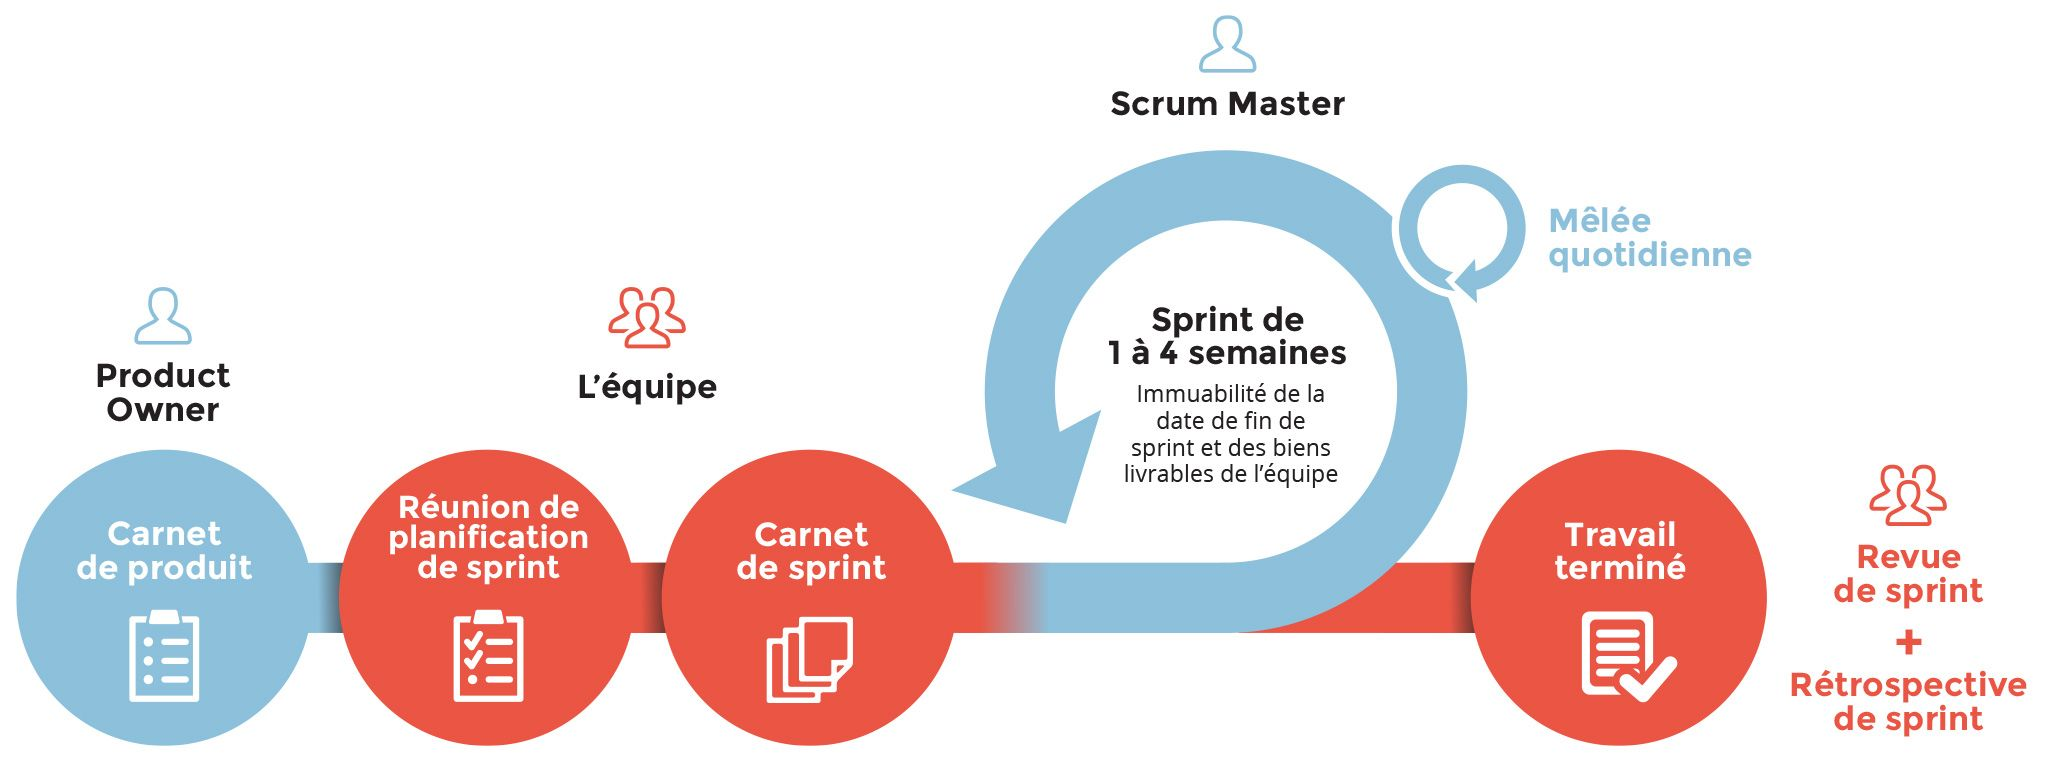
\includegraphics[scale=0.25]{chapitre1/figures/scrum.jpeg}
  \caption{Cycle de vie de en SCRUM}    
  \label{fig:scrum}
\end{figure}




\vspace{5mm}
\subsection{Avantages du modèle SCRUM}
\vspace{5mm}
Parmi les avantages du modèle SCRUM, nous citons : 
\par\vspace{4mm}
\begin{itemize}[label=$\bullet$]
    \item \textbf{Flexibilité et adaptabilité: } SCRUM permet une flexibilité et une adaptabilité constantes, répondant ainsi aux exigences changeantes et assurant l'alignement du produit avec les besoins des parties prenantes.
          \vspace{4mm}
    \item \textbf{Amélioration de la collaboration et de la communication:}  SCRUM favorise une collaboration étroite, une communication régulière et une transparence entre les membres de l'équipe et les parties prenantes, favorisant ainsi la compréhension commune, l'amélioration du travail d'équipe et la résolution rapide des obstacles.
          \vspace{4mm}
    \item \textbf{Délai de mise sur le marché plus court:}   SCRUM permet une livraison rapide et itérative d'incréments de produit utilisables, offrant un retour d'information rapide, des mises à jour incrémentales et une satisfaction client continue.
\end{itemize}
\vspace{5mm}
\subsection{L'équipe SCRUM}
\vspace{5mm}
L’équipe SCRUM est divisée en 3 rôles principaux, qui
interviennent dans le processus de développement du produit, à savoir :
\vspace{6mm}
\begin{itemize}[label=$\bullet$]
\item \textbf{Le Product Owner : } Le Product Owner représente les intérêts du client, définit les besoins du projet, établit les priorités, valide les incréments et participe activement aux réunions de planification et de suivi, assurant ainsi l’alignement avec les attentes et objectifs métier du client.
\vspace{6mm}
\item \textbf{Le SCRUM Master : } Le SCRUM Master assure la bonne mise en oeuvre de la méthode SCRUM,
facilite la résolution des problèmes, agit en tant que coach et favorise la communication et la
collaboration au sein de l’équipe pour atteindre les objectifs du projet.
\vspace{6mm}
\item \textbf{L’équipe de développement SCRUM : } L’équipe de développement SCRUM est une équipe
multidisciplinaire auto-organisée et auto-gérée, responsable de la création et de la réalisation des
fonctionnalités du produit. Elle collabore étroitement, partageant les connaissances et les responsabilités pour atteindre les objectifs du sprint et favoriser une meilleure coordination et efficacité.
\end{itemize}









\newpage
\section{Planification du travail}
\vspace{8mm}

\vspace{8mm}






\begin{table}[ht]
\caption{Diagramme de Gantt}
\centering
\arrayrulecolor{black}
\begin{tabular}{|>{\raggedright\arraybackslash}p{4cm}|>{\centering\arraybackslash}p{1.6cm}|*{16}{>{\centering\arraybackslash}p{0.3cm}|}}
\hline
\multicolumn{1}{|c|}{\textbf{Liste des activités}} & \multicolumn{1}{c|}{\textbf{Janvier}} & \multicolumn{4}{c|}{\textbf{Février}} & \multicolumn{4}{c|}{\textbf{Mars}} & \multicolumn{4}{c|}{\textbf{Avril}} & \multicolumn{4}{c|}{\textbf{Mai}} \\
\hline
\textbf{Semaines} & \textbf{4} & \textbf{1} & \textbf{2} & \textbf{3} & \textbf{4} & \textbf{1} & \textbf{2} & \textbf{3} & \textbf{4} & \textbf{1} & \textbf{2} & \textbf{3} & \textbf{4} & \textbf{1} & \textbf{2} & \textbf{3} & \textbf{4} \\
\hline
\textbf{Analyse et spécification des besoins}  & \cellcolor{blue!50} & \cellcolor{blue!50} & \cellcolor{blue!50} &  &  &  &  &  &  &  &  &  &  &  &  &  &  \\
\hline
\textbf{Conception} &  &  &  & \cellcolor{blue!50} & \cellcolor{blue!50} & \cellcolor{blue!50} &  &  &  &  &  &  &  &  &  &  &  \\
\hline
\textbf{Réalisation} &  &  &  & \cellcolor{blue!50}  & \cellcolor{blue!50}  & \cellcolor{blue!50} & \cellcolor{blue!50} & \cellcolor{blue!50} & \cellcolor{blue!50} & \cellcolor{blue!50} & \cellcolor{blue!50} & \cellcolor{blue!50}  & \cellcolor{blue!50}  & \cellcolor{blue!50}  & \cellcolor{blue!50}  & \cellcolor{blue!50}  & \cellcolor{blue!50}  \\
\hline
\textbf{Élaboration du rapport} &  &  &  & \cellcolor{blue!50}  & \cellcolor{blue!50}  &  &  &  & \cellcolor{blue!50}  &   & \cellcolor{blue!50} & \cellcolor{blue!50} & \cellcolor{blue!50} & \cellcolor{blue!50} & \cellcolor{blue!50} & \cellcolor{blue!50} &  \\
\hline
\end{tabular}
\label{tab:gantt}
\end{table}


\vspace{8mm}

Le diagramme de Gantt présenté dans le tableau \ref{tab:gantt} illustre la planification et la répartition des activités de notre projet sur une période de quatre mois à peu près, de janvier à mai. Les activités principales du projet sont divisées en quatre phases distinctes : l'analyse et la spécification des besoins, la conception, la réalisation et l'élaboration du rapport.

Le tableau permet de visualiser la durée et la séquence de chaque phase du projet. Les cases colorées en bleu indiquent les semaines durant lesquelles une activité spécifique est prévue. Les phases se chevauchent parfois, montrant que certaines activités peuvent être réalisées en parallèle.



















\section{Conclusion}
